\subsection{Glyph: \glyph{Negative influence}}
\label{sec:af:negative_infl}

A \emph{negative influence} is defined as an action that produces a negative or inhibiting effect from one activity to another.

\begin{glyphDescription}

\glyphSboTerm SBO:0000169 ! inhibition

 \glyphOrigin Any \glyph{Activity node} (\sect{af:ANs}) or any \glyph{logical operator} (\sect{af:logic}).
 \glyphTarget Any \glyph{Activity node} (\sect{af:ANs}).
 \glyphEndPoint The target extremity of a \glyph{negative influence} carries a bar perpendicular to the arc (\fig{af:negativeInfl}).


\end{glyphDescription}

\begin{figure}[H]
  \centering
  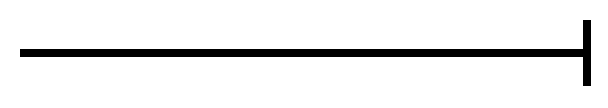
\includegraphics[width = 2in]{images/negativeInfluence}
  \caption{The \AF glyph for \glyph{negative influence}.}
  \label{fig:af:negativeInfl}
\end{figure}



\begin{figure}[H]
  \centering
  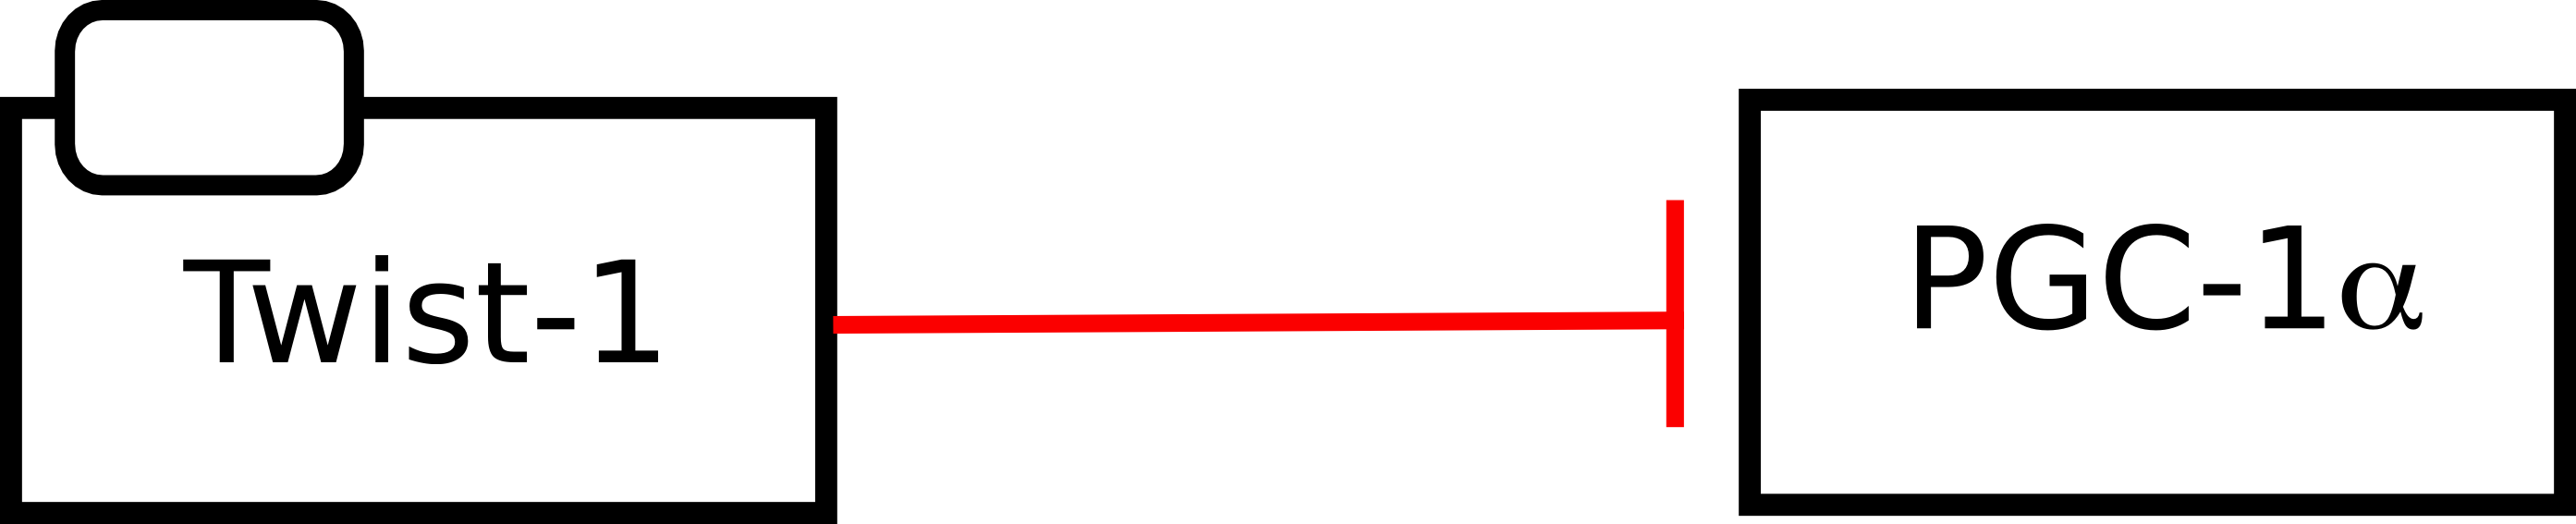
\includegraphics[width = 5in]{examples/ex-negativeInfluence}
  \caption{An example of \glyph{negative influence} from \glyph{"Twist-1"} activity to \glyph{"PGC-1$\alpha$"} activity.}
  \label{fig:af:ex-NI}
\end{figure}